\documentclass[11pt,landscape]{article}
\usepackage[margin=0.75in]{geometry}
\usepackage{tikz}
\usepackage{multicol}
\usepackage{amsmath}
\usepackage{graphicx}
\usepackage{fancyhdr}
\usepackage{array}
\usepackage{tabularx}
\usepackage{helvet} % Use Helvetica font
\renewcommand{\familydefault}{\sfdefault} % Set sans-serif as default
\pagestyle{empty}

\begin{document}

% ---------- TWO-COLUMN LANDSCAPE: FOLDABLE CARD ----------
\noindent
\begin{minipage}[t]{0.48\textwidth}
\raggedright
\Large\textbf{What Kind of Function Is This?} \\
\normalsize
\vspace{1em}

\begin{itemize}
    \item What is \textbf{changing} in this situation?
    \item What is \textbf{staying the same}?
    \item What is the \textbf{input}? What do we control or know?
    \item What is the \textbf{output}? What are we trying to find or measure?
    \item How do the inputs and outputs \textbf{relate}?
    \item Could we represent this situation with a \textbf{table or graph}?
    \item What \textbf{pattern or shape} do we notice when we plot it?
    \item Can we give this rule a \textbf{name}? (\textbf{linear}, \textbf{exponential}, etc.)
    \item Why does this type of function make sense for this context?
\end{itemize}

\vspace{1em}
\textbf{Function Notation:} If $f(x) = 2x + 3$, then $f(4) = 2(4) + 3 = 11$. This is asking: \textit{what is the \textbf{output} when the \textbf{input} is 4?}

\vspace{1em}
\textit{The \textbf{value of the function} is the \textbf{output}—looking for the output in a problem helps you know what shape it is.}

\vspace{2em}
\textit{Somewhere along the way, math changed—}instead of just finding the missing value or solving for \( x \), we started \textbf{modeling problems} and talking about \textbf{multiple ways to represent a situation}. \textbf{That shift is what makes Algebra feel harder—and that’s exactly what we’re going to learn.}

\vspace{2em}

\vfill
\small\textit{Ask yourself: what’s changing, and how? That’s the first step.}
\end{minipage}%
\hfill
\begin{minipage}[t]{0.48\textwidth}
\raggedright
\Large\textbf{Common Function Types on the Regents} \\
\normalsize
\vspace{1em}

\textbf{\underline{Many Regents Questions}}:

\vspace{0.5em}
\begin{tabularx}{\linewidth}{>{\raggedright\arraybackslash}X m{3.2cm}}
\textbf{Linear —} Constant rate of change. Used in cost, distance, and table problems. &
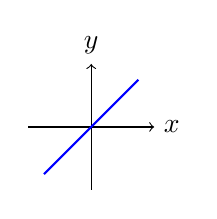
\begin{tikzpicture}[scale=0.4]
\draw[->] (-2,0) -- (2,0) node[right] {$x$};
\draw[->] (0,-2) -- (0,2) node[above] {$y$};
\draw[thick, blue] (-1.5,-1.5) -- (1.5,1.5);
\end{tikzpicture} \\

\textbf{Quadratic —} Parabola shape. Used in height, area, and max/min problems. &
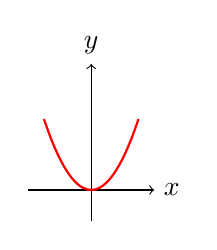
\begin{tikzpicture}[scale=0.4]
\draw[->] (-2,0) -- (2,0) node[right] {$x$};
\draw[->] (0,-1) -- (0,4) node[above] {$y$};
\draw[thick, red, domain=-1.5:1.5, smooth, variable=\x] plot ({\x},{\x*\x});
\end{tikzpicture}
\end{tabularx}

\vspace{1em}
\textbf{\underline{Some Regents Questions}}:

\vspace{0.5em}
\begin{tabularx}{\linewidth}{>{\raggedright\arraybackslash}X m{3.2cm}}
\textbf{Piecewise —} Different \textbf{rules} for different inputs. Graph changes shape. \\ \small $f(x) = \begin{cases} 2x - 3, & x > 3 \\ -x^2 + 15, & x \leq 3 \end{cases}$ &
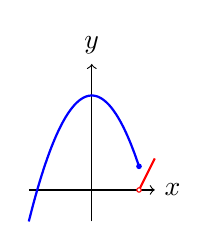
\begin{tikzpicture}[scale=0.4]
\draw[->] (-2,0) -- (2,0) node[right] {$x$};
\draw[->] (0,-1) -- (0,4) node[above] {$y$};
\draw[thick, blue, domain=-2:1.5, smooth, variable=\x] plot ({\x},{-1*\x*\x + 3});
\filldraw[blue] (1.5, -1.5*1.5 + 3) circle (2pt);
\draw[thick, red, domain=1.51:2, smooth, variable=\x] plot ({\x},{2*\x - 3});
\draw[red, fill=white] (1.5, 2*1.5 - 3) circle (2pt);
\end{tikzpicture} \\

\textbf{Absolute Value —} V-shape. Used in comparisons or minimum distance questions. &
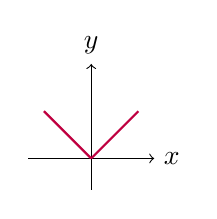
\begin{tikzpicture}[scale=0.4]
\draw[->] (-2,0) -- (2,0) node[right] {$x$};
\draw[->] (0,-1) -- (0,3) node[above] {$y$};
\draw[thick, purple, domain=-1.5:0, smooth] plot (\x,{abs(\x)});
\draw[thick, purple, domain=0:1.5, smooth] plot (\x,{abs(\x)});
\end{tikzpicture} \\

\textbf{Exponential —} Grows or shrinks fast. Used in population or finance. &
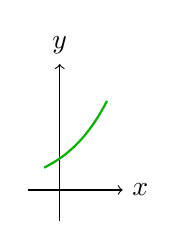
\begin{tikzpicture}[scale=0.4]
\draw[->] (-1,0) -- (2,0) node[right] {$x$};
\draw[->] (0,-1) -- (0,4) node[above] {$y$};
\draw[thick, green!70!black, domain=-0.5:1.5, smooth, variable=\x] plot ({\x},{2^\x});
\end{tikzpicture}
\end{tabularx}

\vfill
\small\textit{Knowing the \textbf{shape} helps you know what to do.}
\end{minipage}

\clearpage

\begin{minipage}[t]{0.48\textwidth}
\raggedright
\Large\textbf{Identifying Change in a Problem Situation} \\
\normalsize
\vspace{0.5em}
When you see a word problem, look for these clues to identify the type of change:

\begin{itemize}
\item What quantity increases or decreases independently?
\item What quantity changes based on something else?
\item Is the change steady (same every time) or changing (faster, slower)?
\item Are we multiplying or adding to get to the next value?
\item Is there a turning point, a break, or a rule change?
\end{itemize}
\end{minipage}
\hfill
\begin{minipage}[t]{0.48\textwidth}
\raggedright
\Large\textbf{Try identifying what is changing in each scenario:} \\
\normalsize
\vspace{0.5em}

\begin{enumerate}
  \item A coffee maker brews one cup every 3 minutes. \\ 
  \small\textit{What quantity is changing?} \normalsize

  \item A YouTube video gains 500 views every hour. \\ 
  \small\textit{Identify the input in this situation.} \normalsize

  \item A population of bacteria doubles every 6 hours. \\ 
  \small\textit{What is the varying quantity?} \normalsize

  \item A bus ride costs \$2 for the first trip, then \$1 for each additional transfer. \\ 
  \small\textit{What drives the total cost?} \normalsize

  \item A washing machine takes 40 minutes per load. A person washes 3 loads back-to-back. \\ 
  \small\textit{What’s the independent variable?} \normalsize

  \item A drone rises, hovers for a few seconds, then descends—all over a span of 15 minutes. \\ 
  \small\textit{Describe what’s changing over time.} \normalsize

  \item A person’s step count is recorded by a smartwatch throughout the day. \\ 
  \small\textit{What’s the domain?} \normalsize

  \item A student earns \$10 for each math worksheet they complete, but gets a bonus after 5. \\ 
  \small\textit{Which quantity is the input?} \normalsize

  \item A remote-controlled car follows a square path around a field, returning to its start. \\ 
  \small\textit{What would the graph of this motion look like?} \normalsize

  \item A medicine’s concentration in the bloodstream decreases at a rate that depends on body weight and metabolism. \\ 
  \small\textit{Identify all potential inputs. Which one is being treated as the domain in most models?} \normalsize
\end{enumerate}
\end{minipage}
\end{document}

